% Created 2016-04-28 Thu 16:52
\documentclass[11pt,xcolor=dvipsnames,presentation]{beamer}
\usepackage[utf8]{inputenc}
\usepackage[T1]{fontenc}
\usepackage{fixltx2e}
\usepackage{graphicx}
\usepackage{longtable}
\usepackage{float}
\usepackage{wrapfig}
\usepackage{rotating}
\usepackage[normalem]{ulem}
\usepackage{amsmath}
\usepackage{textcomp}
\usepackage{marvosym}
\usepackage{wasysym}
\usepackage{amssymb}
\usepackage{hyperref}
\tolerance=1000
\usepackage{minted}
\PassOptionsToPackage{svgnames}{xcolor}
\let\AtBeginDocumentSav=\AtBeginDocument
\def\AtBeginDocument#1{}
\input{org-babel-style-preembule.tex}
\let\AtBeginDocument=\AtBeginDocumentSav
\usepackage{minted}
\usepackage{multirow}
\usetikzlibrary{arrows,shapes,positioning}
\let\tmptableofcontents=\tableofcontents
\def\tableofcontents{}
\usepackage{color,soul}
\definecolor{lightblue}{rgb}{1,.9,.7}
\sethlcolor{lightblue}
\let\hrefold=\href
\renewcommand{\href}[2]{\hrefold{#1}{\SoulColor\hl{#2}}}
\newcommand{\muuline}[1]{\SoulColor\hl{#1}}
\makeatletter
\newcommand\SoulColor{%
\let\set@color\beamerorig@set@color
\let\reset@color\beamerorig@reset@color}
\makeatother
\newcommand{\bottomcitepre}[1]{\fbox{\vbox{\footnotesize #1}}}
\def\mylogos{\\\vspace{1cm}\begin{center}\includegraphics[height=1.2cm]{logos/inr_logo_sans_sign_coul.png}\hspace{0.5cm}\insertlogo{\includegraphics[height=1.2cm]{logos/grid5000.png}}\hspace{0.5cm}\end{center}\vspace{-1cm}}
\usetheme{default}
\usecolortheme{}
\usefonttheme{}
\useinnertheme{}
\useoutertheme{}
\author{Cristian Ruiz, Joseph Emeras, Emmanuel Jeanvoine and Lucas Nussbaum\newline INRIA - France}
\date{May 18, 2016 -- CCGRID 2016 \mylogos}
\title{Distem: Evaluation of Fault Tolerance and Load Balancing Strategies in HPC Runtimes through Emulation}
\hypersetup{
  pdfkeywords={},
  pdfsubject={},
  pdfcreator={Emacs 24.3.1 (Org mode 8.2.10)}}
\begin{document}

\maketitle


\section{}
\label{sec-1}


\begin{frame}[label=sec-1-0-1]{HPC runtimes}
\begin{itemize}
\item According to the IESP report a strong effort must be made on improving HPC software stacks
\item Central part of this stack is the \alert{HPC runtime}
\item HPC runtime enables the execution, managing and debugging of parallel applications
\item OpenMPI, Charm++, CUDA, etc.
\end{itemize}


\alert{For this work we focus on studying HPC runtimes}

\vspace{1cm}
\bottomcitepre{Dongarra, Jack \textit{et Al.},
  {\textit{The International Exascale Software Project Roadmap}},
  International Journal of High Performance Computer Applications,2011}
\end{frame}

\begin{frame}[label=sec-1-0-2]{Evaluating current HPC runtimes}
\begin{block}{Several properties to evaluate}
\begin{itemize}
\item Programability
\item Scalability
\item \alert{Fault tolerance}
\item \alert{Load balancing}
\end{itemize}
\end{block}

\begin{block}{We focus on}
\begin{itemize}
\item Fault tolerance:
more components $\Rightarrow$ shorter MTBF \newline
(Mean Time Between Failures)

\item Load balancing: Cloud computing, Green computing, \newline
  Data centers' policies
\end{itemize}
\end{block}
\end{frame}


\begin{frame}[label=sec-1-0-3]{How people evaluate HPC runtimes?}
Some examples

\begin{itemize}
\item Ad-hoc simulator and real application trace from IBM BG/Q
\end{itemize}
\bottomcitepre{Harshitha Menon and L. V. Kalew,
  {\textit{A Distributed Dynamic Load Balancer for Iterative Applications}},
  SC'2013}

\begin{itemize}
\item Leveraging DVFS processor capabilities
\end{itemize}
\bottomcitepre{Osman Sarood \textit{et Al.},
  {\textit{A 'Cool' Way of Improving the Reliability of HPC Machines}},
  SC'2013}
\begin{itemize}
\item For MPI based runtimes, most of the experiments are done using real platforms
\end{itemize}
\end{frame}
\begin{frame}[label=sec-1-0-4]{Evaluating current HPC runtimes}
\begin{itemize}
\item Carrying out evaluation under complex realistic conditions is \alert{hard}
\item Simulator:
\begin{itemize}
\item simplified assumptions $\frowny$
\item lower realism $\frowny$
\item not possible to run a complete software stack $\frowny$
\end{itemize}

\item Real platform:
\begin{itemize}
\item expensive $\frowny$
\item lacks of reproducibility $\frowny$
\end{itemize}
\end{itemize}
\end{frame}


\section{Distem}
\label{sec-2}
\let\tableofcontents=\tmptableofcontents
\AtBeginSection[]
  {
     \begin{frame}<beamer>
     \frametitle{Outline}
     \tableofcontents[currentsection]
     \end{frame}
  }
\input{org-babel-document-preembule.tex}

\begin{frame}[label=sec-2-0-1]{Distem}
\begin{center}
\huge
An emulator for distributed systems\\[0.5em]
\large
Take your \alert{real application}\\[0.5em]
Run it on a \alert{cluster}\\[0.5em]
And use \alert{Distem} to \alert{alter the platform}\\
so it \alert{matches the experimental conditions you need}\\[1em]
\normalsize
\begin{tikzpicture}
\pgftext[right]{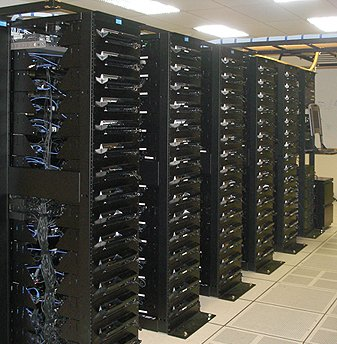
\includegraphics[width=3cm]{figures/cluster.jpg}}
\draw[line width=1.5mm] (0.1, 0) -- (0.9, 0);
\draw[line width=1.5mm] (0.5, -0.4) -- (0.5, 0.4);
\pgftext[x=1.25cm,left]{
\includegraphics[width=2.5cm]{figures/distem.png}}
\draw[line width=1.5mm,->] (4.1,0) -> (4.9,0);
\begin{scope}[xshift=2cm]
\pgftext[x=5cm,y=0.75cm,center]{Heterogeneous nodes}
\pgftext[x=5cm,y=0.25cm,center]{Long distance networks}
\pgftext[x=5cm,y=-0.25cm,center]{Faults, perf. variations}
\pgftext[x=5cm,y=-0.75cm,center]{Grid, Cloud, P2P features}
\pgftext[x=5cm,y=-1.25cm,center]{\Large\ldots}
\end{scope}
\end{tikzpicture}
\end{center}
\end{frame}



\begin{frame}[label=sec-2-0-2]{Distem features}
The features of Distem include:

\begin{itemize}
\item running many virtual nodes on each physical node
\item emulation of CPU performance, network topologies, IO speed
\end{itemize}

Distem uses modern Linux functionality:

\begin{itemize}
\item Linux containers
\item control groups
\item CPU frequency scaling
\item traffic control
\item I/O throttling
\end{itemize}
\end{frame}

\begin{frame}[label=sec-2-0-3]{In this work}
We integrated the following improvements in order to
make possible the evaluation of HPC runtimes:

\begin{itemize}
\item Evolving experimental conditions
\item Failure injection framework
\item Event injection framework
\end{itemize}
\end{frame}

\begin{frame}[label=sec-2-0-4]{Evolving experimental conditions}

\begin{minipage}{0.5\textwidth}
\begin{center}
    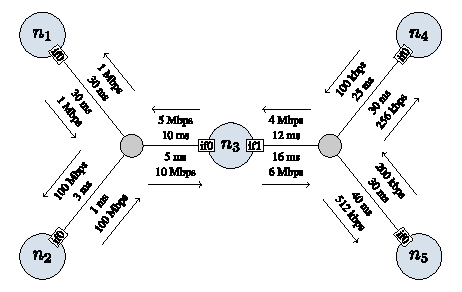
\includegraphics[width=0.9\textwidth]{figures/links}
\end{center}\end{minipage}\hfill
\begin{minipage}{0.5\textwidth}
\begin{center}
    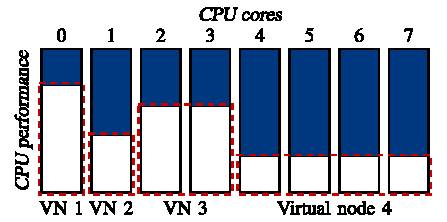
\includegraphics[width=\textwidth]{figures/procs}
\end{center}\end{minipage}

\begin{itemize}
\item Heterogeneous conditions can be created: CPU frequencies,
different IO and network capabilities

\item These features can be updated dynamically

\item This is useful to achieve complex experiments where the platform is modified,
like it could happened in reality
\end{itemize}
\end{frame}

\begin{frame}[label=sec-2-0-5]{Failure injection framework}

\begin{itemize}
\item We take into account failures that provoke a lost of the node (very common failures)

\item Nodes can be lost in three different ways:

\begin{itemize}
\item \alert{Graceful}: the node is shut down cleanly, using an operating system command
\item \alert{Soft}: the node is forced to shut down
\item \alert{Hard}: the node failed abruptly
\end{itemize}

\item We do not take into account byzantine failures
\end{itemize}
\end{frame}

\begin{frame}[label=sec-2-0-6]{Event injection framework}
\begin{itemize}
\item Increase the reproducibility of experiments
\item Distem supports the following modifications for a given set of nodes:
\begin{itemize}
\item CPU frequency
\item Network capabilities (latency and bandwidth)
\item Failures
\end{itemize}
\item These modifications can be injected using a deterministic behavior or using
a probabilistic distribution
\end{itemize}
\end{frame}


\section{Experimental results}
\label{sec-3}
\begin{frame}[label=sec-3-0-1]{Experiment setup}
\begin{itemize}
\item We evaluate Charm++, OpenMPI and MPICH runtimes
\item Charm++: Jacobi3D and Stencil3D
\item MPI-based runtimes:  NAS parallel benchmarks

\item 3 Grid'5000 clusters located in two sites

\item Experimental evaluation:
\begin{itemize}
\item \emph{Failure detection of HPC runtimes}
\item \emph{Validity of fault injection mechanism}
\item \emph{Evaluation of load balancing strategies in Charm++}
\end{itemize}
\end{itemize}
\end{frame}

\begin{frame}[label=sec-3-0-2]{Failure detection of HPC runtimes}
\begin{itemize}
\item We run an application on top of the HPC runtime
\item We inject different types of faults and observe how the HPC runtime reacts
\end{itemize}


\begin{table}[ht!]
  { \scriptsize
  \begin{tabular}{|c|c|c|c|c|c|c|}
  \hline
  \multirow{3}{*}{\textbf{Failure}} &
  \multicolumn{6}{c|}{\textbf{Runtime}}  \\
  \cline{1-7}
  &\multicolumn{2}{c}{\textbf{Charm++}}&
  \multicolumn{2}{|c}{\textbf{OpenMPI}}&
  \multicolumn{2}{|c|}{\textbf{MPICH}}\\
  \cline{2-7}
  &\textbf{Detected} & \textbf{Action} & \textbf{Detected} & \textbf{Action} & \textbf{Detected} & \textbf{Action}  \\
  \hline
  \textbf{Graceful}  &   Yes  & C   &  Yes   &  \color{red}{H}  &  Yes   &  E   \\
  \textbf{Soft}  &       Yes  & C   &  Yes   &  \color{red}{H}  &  Yes   &  E   \\
  \textbf{Hard}   &      \color{red}{No}   & -   &  Yes   &  \color{red}{H}  &  Yes   &  E   \\
  \hline
  \end{tabular}
  }
  \caption{Failure detection. C refers to the roll-back of the application to the previous checkpoint,
  H refers to the fact that processes hang, E refers to the termination of MPI processes}
  \label{table:assess_HPC_runtimes}
\end{table}
\end{frame}

\begin{frame}[label=sec-3-0-3]{Validity of fault injection mechanism}
\begin{itemize}
\item We run Jacobi3D application using 64 nodes, running 1 Charm++ process per node

\item Different degrees of oversubscription

\item We use the event injection framework to inject the same trace for all cases
\end{itemize}

\begin{table}[ht!]
        \center
  {\scriptsize
  \begin{tabular}{|c|c|c|}
  \hline
    \textbf{Mechanism}  &  \textbf{ \% termination} & \textbf{ Mean walltime
    (secs)} \\
  \hline
  \textbf{Charm++ Injection}  &  \color{red}{100\%} & 268.55\\
  \textbf{Real Injection}  &  66\% & 267.19\\
  \textbf{Distem 1vn/node}  &  56\% & 286.43\\
  \textbf{Distem 2vn/node}  &  50\% & 287.05\\
  \textbf{Distem 4vn/node}  &  56\% & 294.45\\
  \hline
  \end{tabular}
  }
  \caption{Percentage of successful application executions}
  \label{table:FT_validation}
\end{table}
\end{frame}

\begin{frame}[label=sec-3-0-4]{Evaluating load balancing strategies in Charm++}
\begin{itemize}
\item We create a platform composed 128 vnodes distributed over 8 physical nodes.

\item We experiment with two different scenarios:

\begin{itemize}
\item \alert{Heterogeneous}: half of the vnodes have a CPU clock reduced to 50 \%

\item \alert{Dynamic}: the available CPU power of a sub-part of the vnodes is dynamic.
\end{itemize}
\end{itemize}


The event injection framework was used to automate the creation of these scenarios
\end{frame}

\begin{frame}[label=sec-3-0-5]{Evaluating load balancing strategies in Charm++}
Running Stencil3D using 128 processes in the heterogeneous platform

\vspace{0.5cm}
\begin{minipage}{0.30\textwidth}
\begin{center}
\begin{figure}
    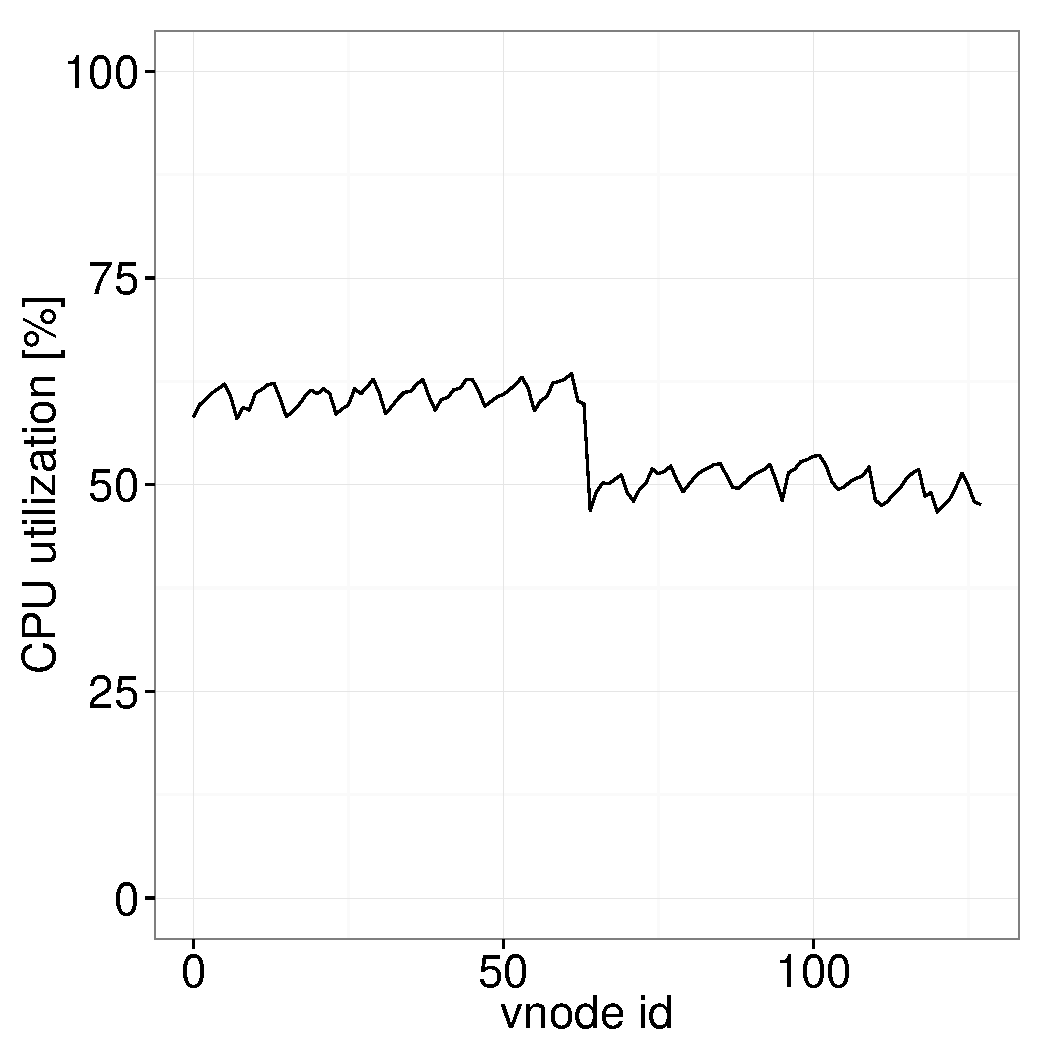
\includegraphics[scale=0.22,angle=0]{figures/usage-heterogeneous.pdf}
    \caption{\centering LBOff \newline Walltime: 341 secs}
    \label{fig:heterogeneous}
\end{figure}
    \end{center}\end{minipage}\hfill
\begin{minipage}{0.3\textwidth}
    \begin{center}
\begin{figure}
    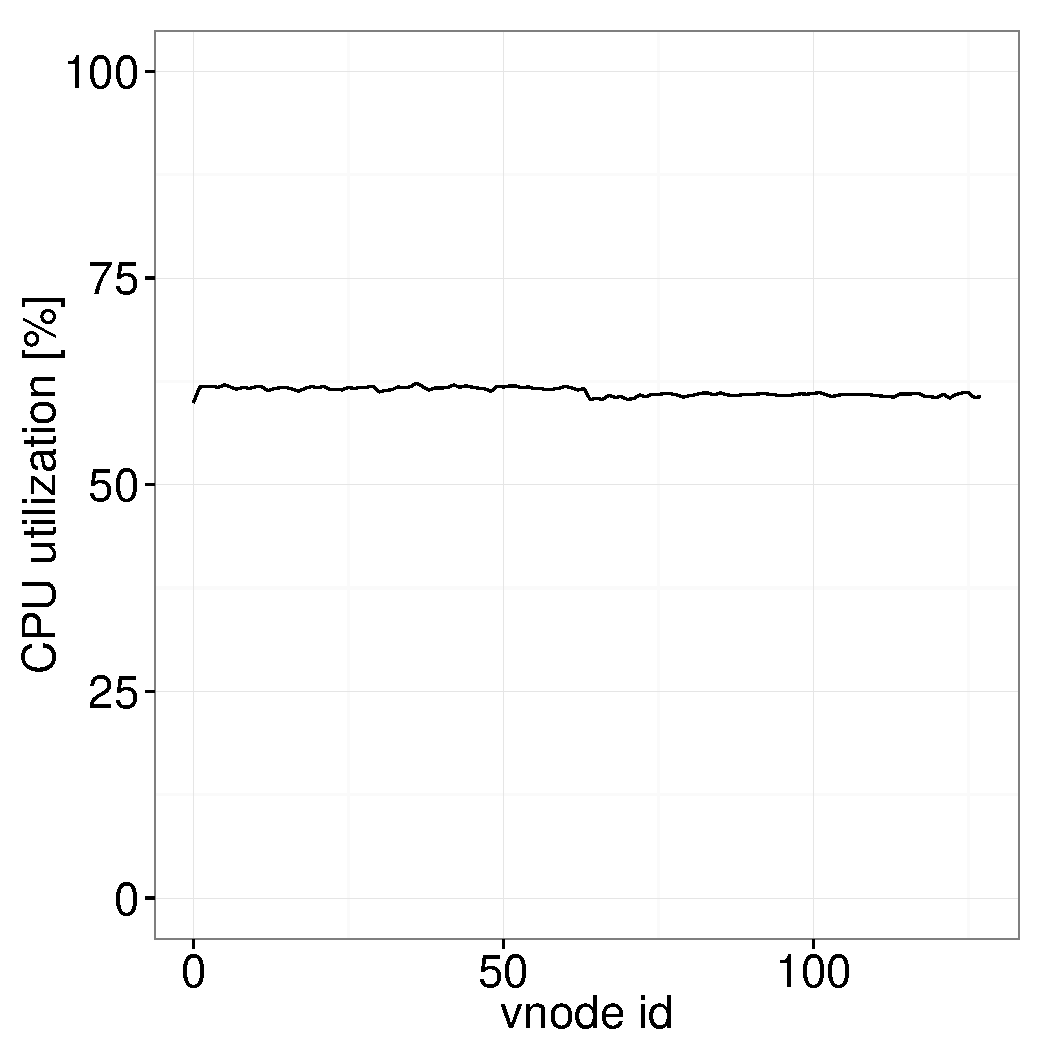
\includegraphics[scale=0.22,angle=0]{figures/usage-heterogeneous_refinelb.pdf}
   \caption{\centering RefineLB \newline Walltime: 320 secs}
    \label{fig:refinelbh}
\end{figure}
\end{center}\end{minipage}\hfill
    \begin{minipage}{0.3\textwidth}
    \begin{center}
\begin{figure}
    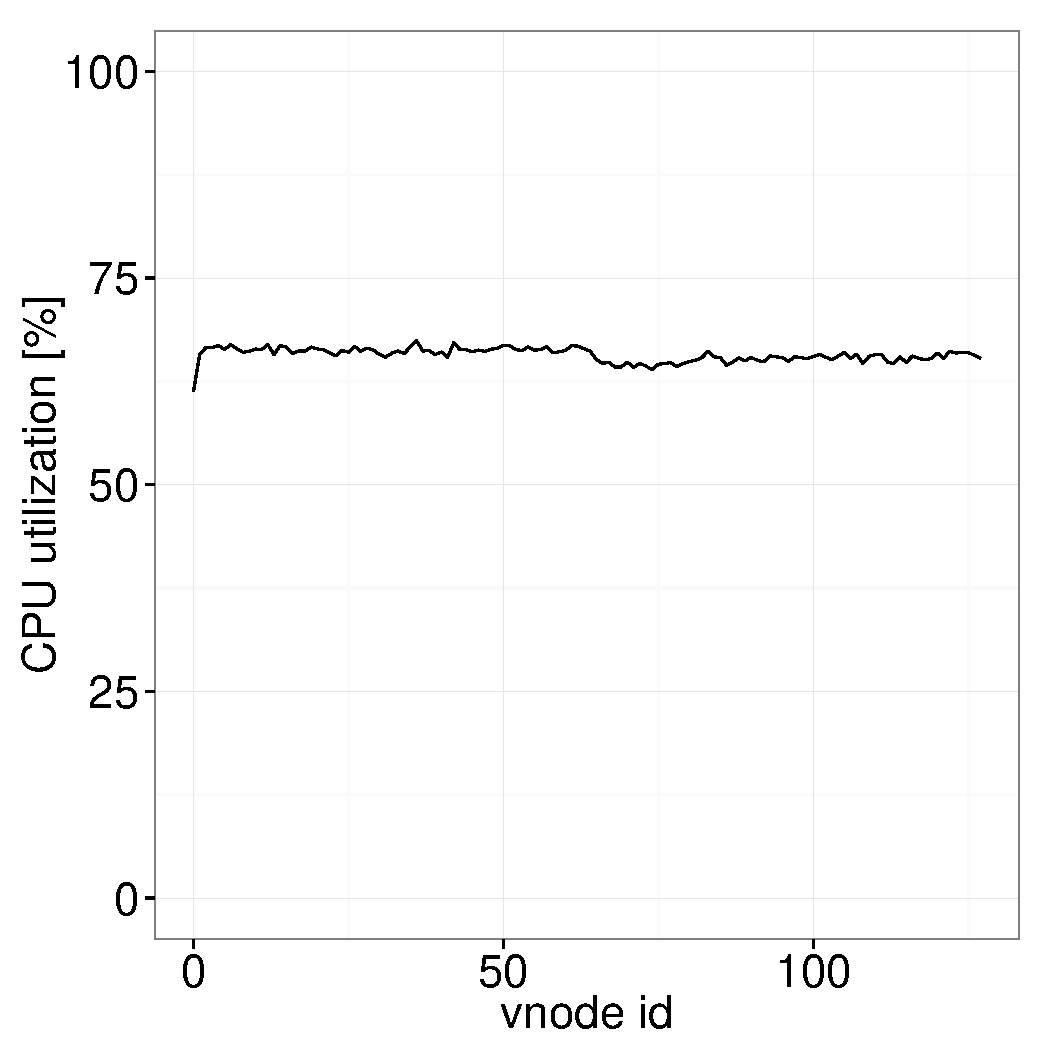
\includegraphics[scale=0.22,angle=0]{figures/usage-heterogeneous_hybrid}
    \caption{\centering Hybrid \newline Walltime: 356 secs}
        \label{fig:hybridlbh}
\end{figure}
    \end{center}\end{minipage}
\end{frame}

\begin{frame}[label=sec-3-0-6]{Evaluating load balancing strategies in Charm++}
Running Stencil3D using 128 processes in the dynamic platform

\vspace{0.5cm}
\begin{minipage}{0.30\textwidth}
\begin{center}
\begin{figure}
    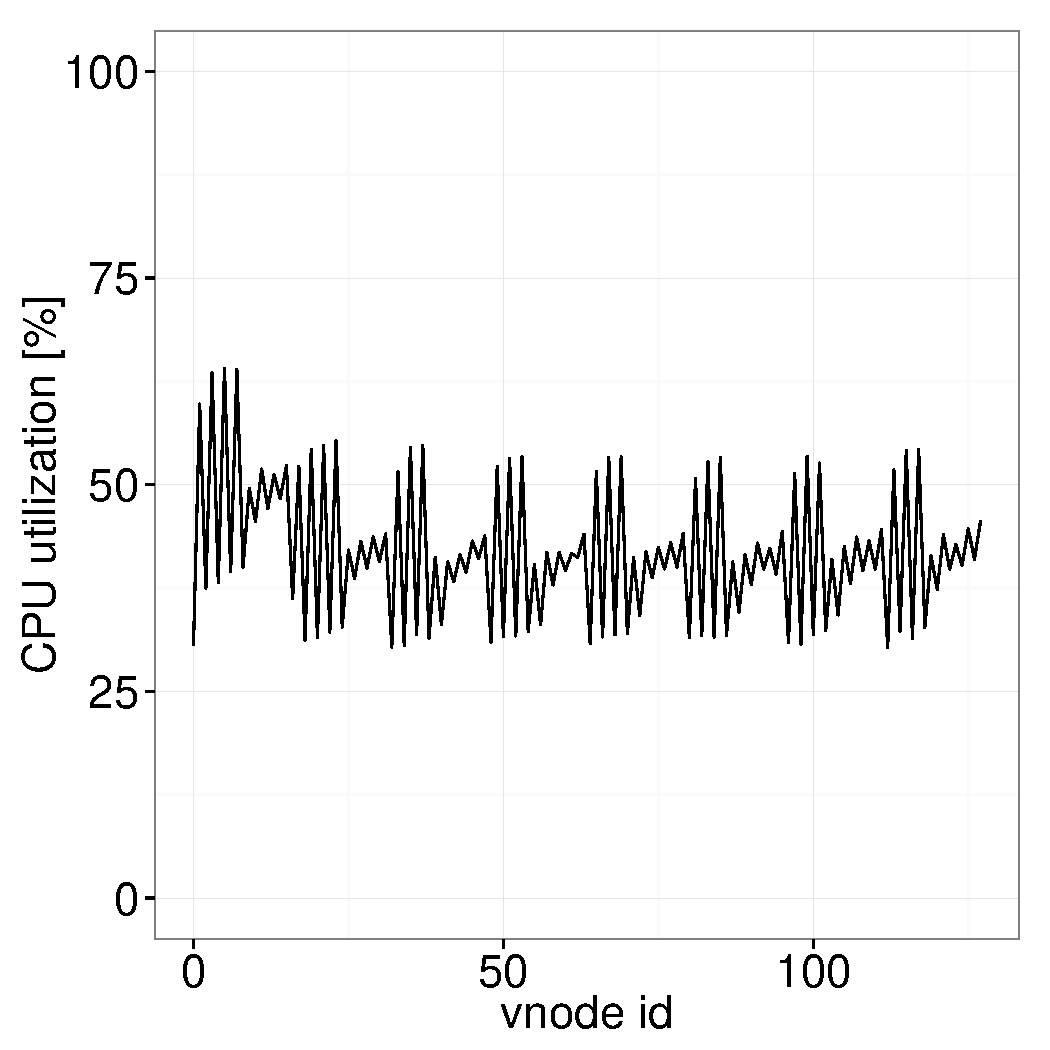
\includegraphics[scale=0.22,angle=0]{figures/usage-dynamic}
    \caption{\centering LBOff \newline Walltime: 347 secs}
    \label{fig:heterogeneous}
\end{figure}
    \end{center}\end{minipage}\hfill
\begin{minipage}{0.3\textwidth}
    \begin{center}
\begin{figure}
    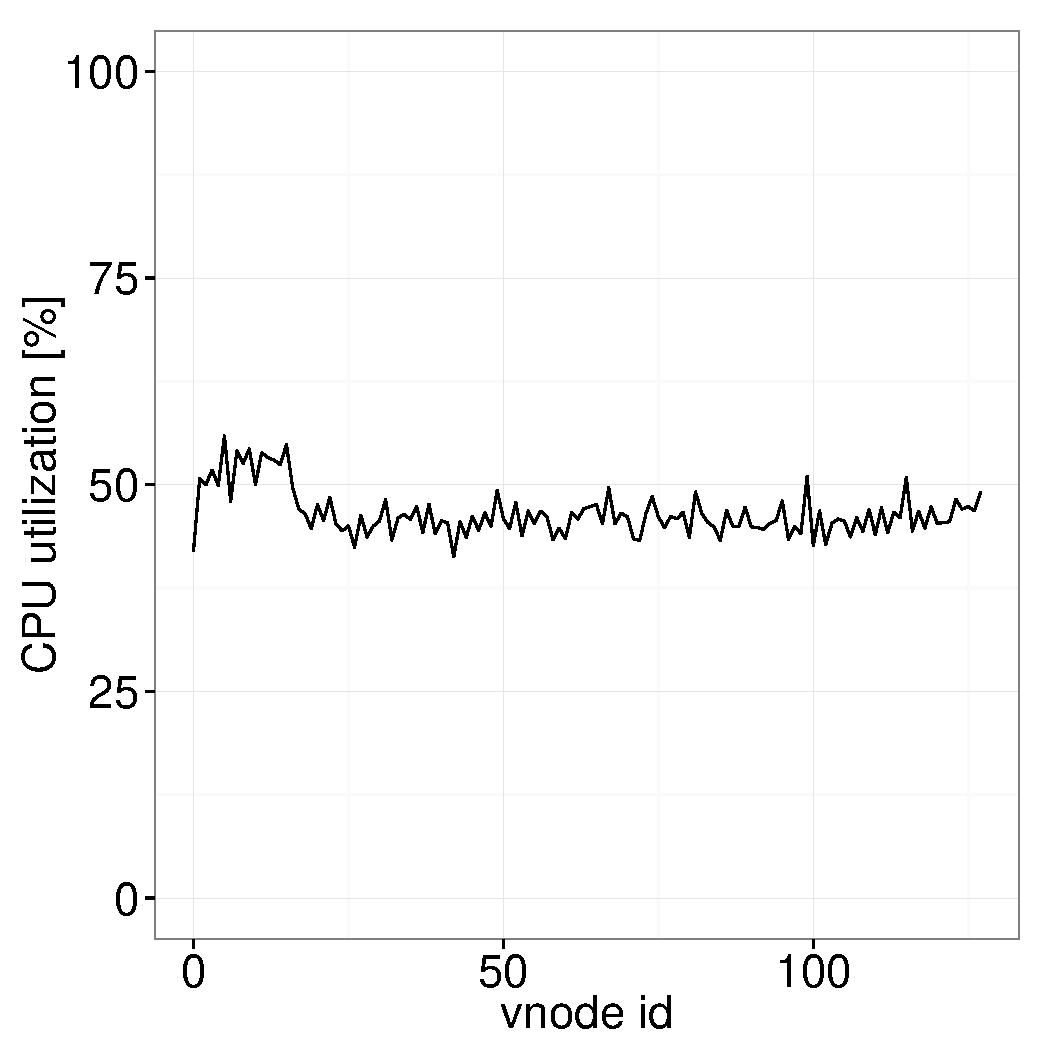
\includegraphics[scale=0.22,angle=0]{figures/usage-dynamic_refinelb}
   \caption{\centering RefineLB \newline Walltime: 322 secs}
    \label{fig:refinelbh}
\end{figure}
\end{center}\end{minipage}\hfill
    \begin{minipage}{0.3\textwidth}
    \begin{center}
\begin{figure}
    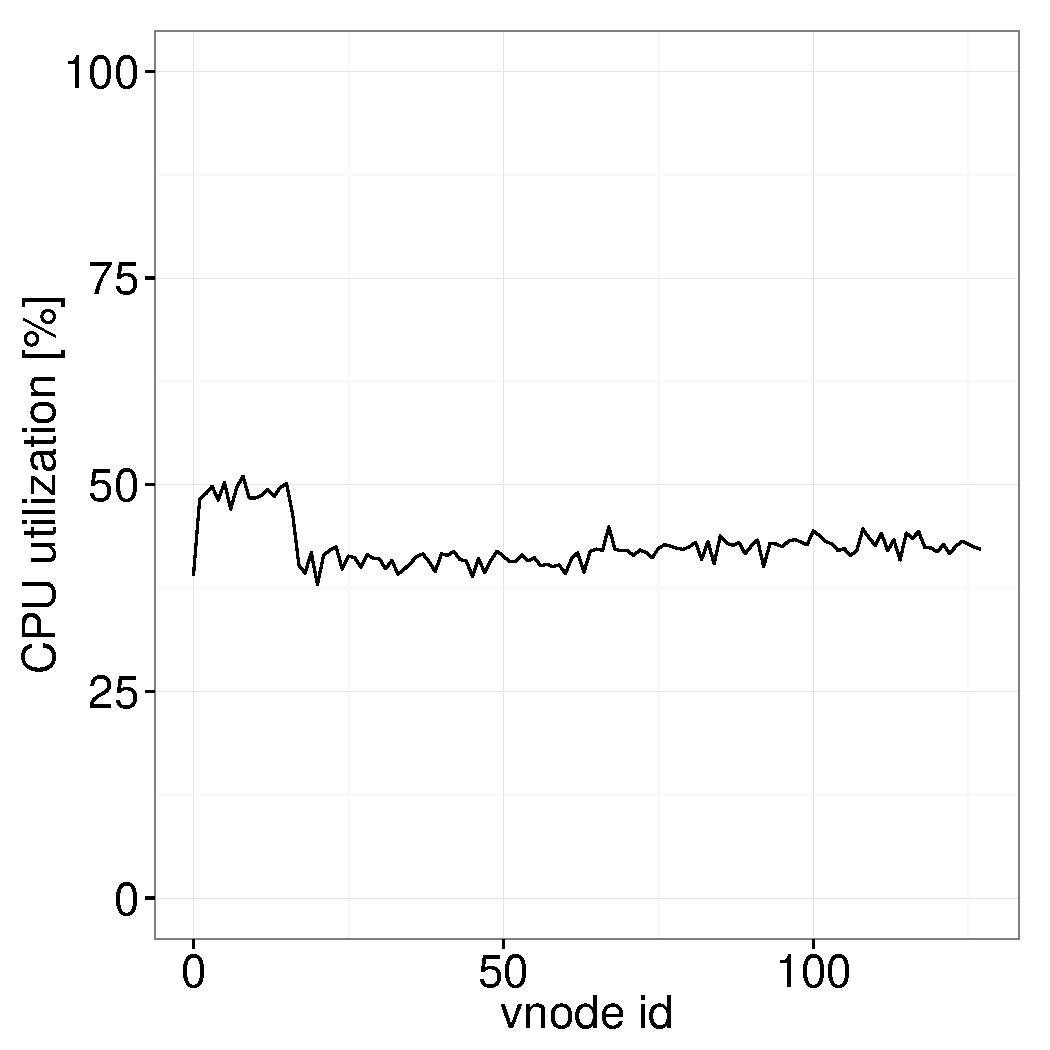
\includegraphics[scale=0.22,angle=0]{figures/usage-dynamic_hybrid}
    \caption{\centering Hybrid \newline Walltime: 359 secs}
        \label{fig:hybridlbh}
\end{figure}
    \end{center}\end{minipage}
\end{frame}


\section{Conclusions}
\label{sec-4}

\begin{frame}[label=sec-4-0-1]{Conclusions}
\begin{itemize}
\item Being able to execute experiments on a large set of platform
configurations in a repeatable way is a sound basis to design
and improve the HPC runtimes in the future
\end{itemize}

\vspace{0.5cm}
\begin{itemize}
\item \alert{Distem:}
\begin{itemize}
\item offers realistic experimental conditions

\item simplified the uncovering of problems in the
failure handling for widely used HPC runtimes

\item enables experimenters to easily simulate perturbations and
heterogeneity of nodes
\end{itemize}
\end{itemize}
\end{frame}
% Emacs 24.3.1 (Org mode 8.2.10)
\end{document}
